\renewcommand{\SourceFile}{6-geometrie-et-images/src/6-4.ml}

\section{Polygones convexes}

Nous définissons un point de l'écran (que l'on considère muni d'un repère orthonormé direct) comme étant un couple d'entiers $(x,y)$, et un polygone comme étant une suite finie de points telle que tout couple formé de deux points consécutifs ou du dernier et du premier point de cette suite représente une arête du polygone.
\medskip

Nous supposons qu'il n'y a \textbf{pas de points consécutifs alignés}.
\medskip

Attention : nous ne disposons pas de fonctions trigonométriques.

\Q
Écrire la fonction OCaml \texttt{saillant} qui prend trois points $A$, $B$ et $C$ comme arguments et qui renvoie \texttt{true} si la mesure de l'angle $(BA,BC)$, suivant le sens trigonométrique, est inférieure à $180$\textdegree{} et \texttt{false} sinon.

\Q
Pour tester si un polygone est convexe, on vous propose la méthode suivante : soient \texttt{p} un polygone et $n$ le nombre de sommets \texttt{p.(i)} (pour \texttt{i} entre 0 et $n-1$) de celui-ci. Si pour tout triplet (\texttt{p.(i)}, \texttt{p.(i+1 mod n)}, \texttt{p.(i+2 mod n)}) on tourne dans un même sens (pour \texttt{i} entre 0 et $n-1$) alors le polygone est convexe, sinon il ne l'est pas. Implémenter cette méthode par une fonction OCaml \texttt{tester} qui utilise la fonction \texttt{saillant}. Évaluer le nombre d'appels à la fonction \texttt{saillant} lors de l'exécution de la fonction \texttt{tester}. La réponse est-elle toujours correcte ?

\Q
Modifier la fonction \texttt{tester} sans en augmenter le nombre d'appels à \texttt{saillant}, de façon qu'elle renvoie toujours une réponse correcte.

\Q
Considérons un ensemble $E$ de points. Écrire une fonction \texttt{enveloppe} qui renvoie l'enveloppe convexe de $E$. Évaluer le nombre d'appels à la fonction \texttt{saillant}.

\Q
Supposons l'ensemble $E$ tel que son premier point est celui d'ordonnée minimale et les points suivants sont ordonnés suivant les angles polaires croissants avec \texttt{e.(0)} comme origine. Écrire une fonction de balayage telle que le nombre d'appels à la fonction \texttt{saillant} est de l'ordre de grandeur du nombre de points de l'ensemble $E$.

\Corrige

\Q
Nous utilisons les structures de données suivantes :

\lstinputlisting[linerange={1-2}]{\SourceFile}

La fonction \texttt{saillant} s'écrit simplement.
\medskip

On utilise le fait que : $\det(u,v)=||u||\cdot||v||\cdot\sin(u,v)$.

\lstinputlisting[linerange={4-7}]{\SourceFile}

\Q
Nous appliquons l'algorithme proposé dans l'énoncé.

\lstinputlisting[linerange={9-21}]{\SourceFile}

La fonction \texttt{saillant} est appelée au plus $n+1$ fois. Cette fonction ne tient compte que du sens de rotation lorsque l'on passe d'un sommet à son suivant, or il peut y avoir une intersection qui rompt la convexité (voir dessin).

\begin{center}
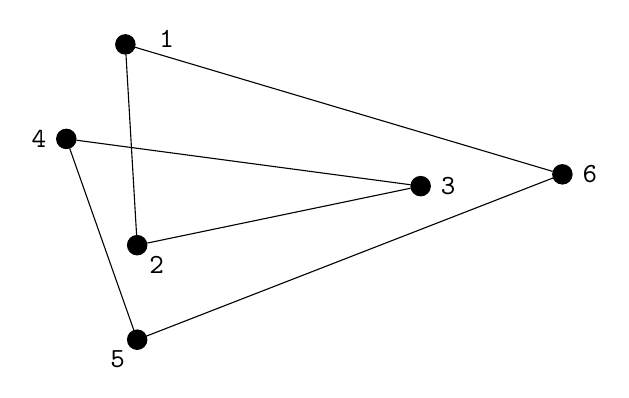
\begin{tikzpicture}[scale=1.5,
    label distance=2pt,
    every node/.style={
    font=\ttfamily,
    draw,
    fill=black,
    circle,
    inner sep=0pt,
    minimum size=7pt}]

    \node[label={[xshift=5pt, yshift=2pt]right:1}] (1) at (.5,2.8) {};
    \node[label=below right:2] (2) at (.6,1.1) {};
    \node[label=right:3] (3) at (3,1.6) {};

    \node[label=left:4] (4) at (0,2) {};
    \node[label=below left:5] (5) at (.6,.3) {};
    \node[label=right:6] (6) at (4.2,1.7) {};

    \draw (1) -- (2) -- (3) -- (4) -- (5) -- (6) -- (1);
\end{tikzpicture}
\end{center}

\Q
Afin de tester s'il y a une intersection, on compte le nombre de changements de direction suivant les abscisses lorsque l'on parcourt les sommets consécutifs du polygone considéré. Compte tenu du fait que l'on tourne toujours dans le même sens, si ce nombre est strictement inférieur à 3 alors il n'y a pas d'intersection. Dans ce cas, pour chaque arête considérée, tous les sommets sont d'un même côté, ce qui définit bien un polygone convexe.

\lstinputlisting[linerange={23-39}]{\SourceFile}

\Q
On part du point de l'ensemble $E$ d'ordonnée la plus basse, ce point est le premier sommet de l'enveloppe convexe $P$. Puis on cherche le point $M$ de l'ensemble $E$ tel que si on passe en argument de la fonction \texttt{saillant} le segment d'extrémités le dernier sommet de $P$ et $M$, et un point quelconque de $E$ alors \texttt{saillant} renvoie \texttt{true}. On ajoute ce point à l'enveloppe convexe $P$ puis on recommence en partant du point suivant dans $E$. L'algorithme s'arrête dès que l'on revient sur le premier point de $P$.

\lstinputlisting[linerange={40-61}]{\SourceFile}

\Q
Les points de $E$ sont classés par ordre croissant d'angle polaire avec comme origine le point le plus bas de $E$. On place d'office les trois premiers points de $E$ dans $P$. Puis, on considère le point suivant : si ce point et les deux derniers de $P$ forment un angle saillant, on ajoute ce point à $P$, sinon, on retire le dernier point de $P$ et on recommence ce test. On parcourt ainsi tous les points de $E$.

\lstinputlisting[linerange={63-77}]{\SourceFile}

La fonction \texttt{saillant} est appelée au plus $2n-3$ fois.
\bigskip

\Fin
